%================================================================================================
%================================= PRIMEIRA FOLHA INTERNA  ======================================
%================================================================================================
\begin{figure}
\center

\includegraphics[height=0.15\textwidth]{Figs/logoCefetCampusPetropolis.jpg} 
\end{figure}


\vspace*{0.8cm}

\begin{center}
{\large \bf CENTRO FEDERAL DE EDUCAÇÃO TECNOLÓGICA} \vspace{1mm} \\
{\large \bf CELSO SUCKOW DA FONSECA - CEFET/RJ \textit{CAMPUS} PETRÓPOLIS} \vspace{1mm} \\
{\large \bf CURSO: BACHARELADO EM ENGENHARIA DE COMPUTAÇÃO}\\

\vspace*{5cm}
{\large \bf \blue{[ToDo:] Título do trabalho.}}\\
\end{center}
\vspace{4cm}
\hfill
%\begin{minipage}%{0.45\linewidth}
	\begin{flushright}
	{ Jonatas Halliday Sant Anna do Nascimento}
	\end{flushright}
%\end{minipage}


\vspace*{3.3cm}
\begin{center}
{\bf PETRÓPOLIS \\{ 2026}}\\
\end{center}

%--------------------------------------------------------------------------
%--------------------------------------------------------------------------
\newpage
\pagestyle{empty}

\begin{center}
{\large \bf CENTRO FEDERAL DE EDUCAÇÃO TECNOLÓGICA} \vspace{1mm} \\
{\large \bf CELSO SUCKOW DA FONSECA - CEFET/RJ \textit{CAMPUS} PETRÓPOLIS} \vspace{1mm} \\
{\large \bf CURSO: BACHARELADO EM ENGENHARIA DE COMPUTAÇÃO}

\vspace*{3cm}
\normalsize{\large \bf \blue{[ToDo:] Título do trabalho.}}\\
\end{center}
\vspace{1.5cm}
\hfill
%\begin{minipage}%{0.45\linewidth}
	\begin{flushright}
	\blue{Jonatas Halliday Sant Anna do Nascimento}
	\end{flushright}
%\end{minipage}
\vspace*{1.5cm}
\begin{flushright}
	\begin{minipage}{0.5\textwidth}
		{\normalsize
		Trabalho de Conclusão de Curso apresentado ao  
	 CEFET/RJ - {\it campus} Petrópolis, como parte dos requisitos para obtenção do título de Bacharel em Engenharia de Computação.}
	\end{minipage}\\[1.5cm]
\end{flushright}
\vspace{1.5cm}
\hfill
%\begin{minipage}%{0.45\linewidth}
\begin{flushright}
\blue{[ToDo:] Orientadora: Professor(a) Nome do Professor(a)}\\
\blue{[ToDo:] Coorientador: Professor(a) Nome do Professor(a)}
\end{flushright}




\vspace*{3.3cm}
\begin{center}
{\bf PETRÓPOLIS \\ \blue{[ToDo:] Ano}}\\
\end{center}



%--------------------------------------------------------------------------
%--------------------------------------------------------------------------
\newpage
\begin{minipage}{0.9\textwidth}

{\normalsize 
\begin{center}
Autorizo a reprodução e divulgação total ou parcial deste trabalho, por qualquer meio eletrônico ou convencional, para fins de estudo e pesquisa, desde que citada a fonte.
\end{center}
\vspace*{0.5cm}
}
\end{minipage}
\vspace*{5cm}
\begin{center}
\blue{[ToDo:] Acrescentar ficha catalográfica (providenciada pela biblioteca) após a defesa do TCC.}
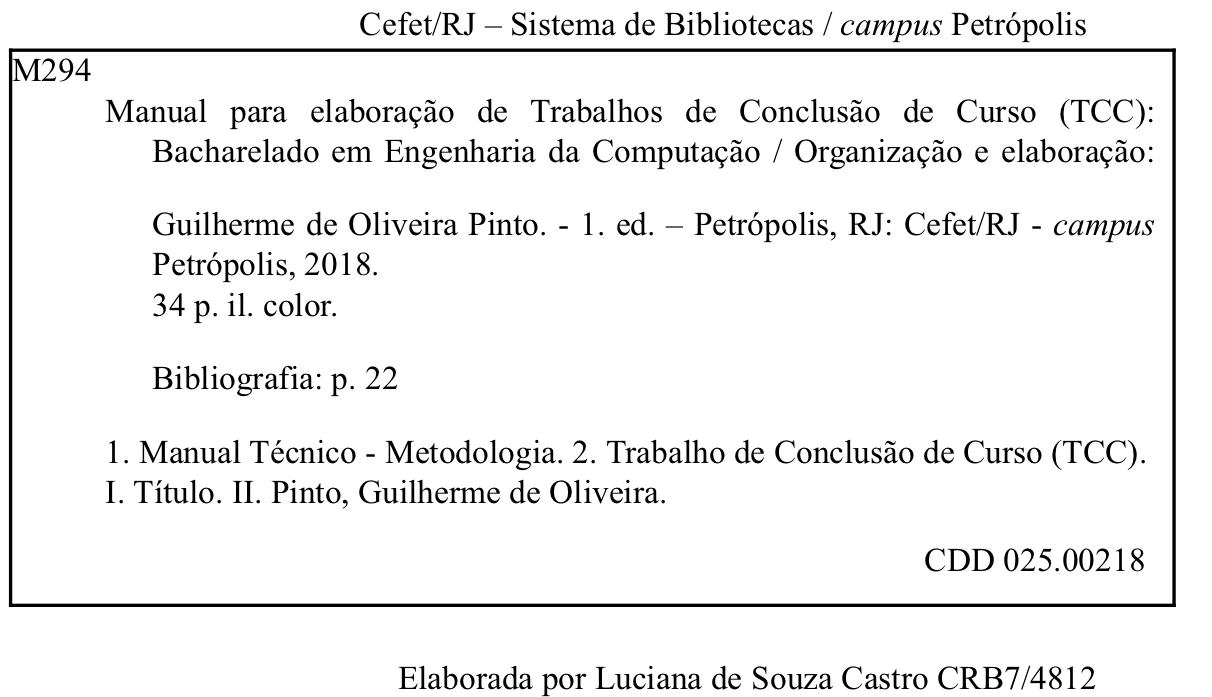
\includegraphics[height=0.5\textwidth]{Figs/biblioteca_engcomp.jpeg}
\end{center}


%--------------------------------------------------------------------------
%--------------------------------------------------------------------------

\newpage
\newcommand{\HRule}{\rule{0.6\linewidth}{0.5mm}}
\pagestyle{empty}

{\center % Center everything on the page


\begin{figure}
\center

\includegraphics[height=0.13\textwidth]{Figs/logoCefetCampusPetropolis.jpg} 
\end{figure}

\begin{center}
{\large \bf CENTRO FEDERAL DE EDUCAÇÃO TECNOLÓGICA} \vspace{1mm} \\
{\large \bf CELSO SUCKOW DA FONSECA - CEFET/RJ \textit{CAMPUS} PETRÓPOLIS} \vspace{1mm} \\
{\large \bf CURSO: BACHARELADO EM ENGENHARIA DE COMPUTAÇÃO}\\
\vspace*{1.2cm}
{\large  FOLHA DE APROVAÇÃO}

\vspace*{1.3cm}
{\large \bf \blue{[ToDo:] Título do trabalho.}}\\
\end{center}
\vspace{0.5cm}
\hfill
%\begin{minipage}%{0.45\linewidth}
\begin{flushright}
    \blue{Jonatas Halliday Sant Anna do Nascimento}
	\end{flushright}
%\end{minipage}
\vspace*{0.5cm}
\begin{flushright}
	\begin{minipage}{0.5\textwidth}
		{\normalsize
		Trabalho de Conclusão de Curso apresentado ao  
	 CEFET/RJ -{ {\it campus} Petrópolis}, como parte dos requisitos para obtenção do título de Bacharel em Engenharia de Computação.}
	\end{minipage}\\[0.5cm]
\end{flushright}
\vspace{0.5cm}
\hfill
%\begin{minipage}%{0.45\linewidth}
\begin{flushright}
\blue{[ToDo:] Orientador(a): Nome do Professor(a)} \\
\blue{[ToDo:] Corientador(a): Nome do Professor(a)} \\
\end{flushright}

\begin{minipage}{0.9\textwidth}
	\begin{flushleft}
	Aprovado por:
	\end{flushleft}
\end{minipage}\\[1cm]

\center
\HRule \\
\blue{[ToDo:] Nome do Professor(a)} \\[0.4cm]
\HRule \\
\blue{[ToDo:] Nome do Professor(a)} \\[0.4cm]
\HRule \\
\blue{[ToDo:] Nome do Professor(a)} \\[0.4cm]
\HRule \\
\blue{[ToDo:] Nome do Professor(a)} \\[1.2cm]


\begin{center}
\blue{[ToDo:] Mês de Ano}
\end{center}


}



\newpage


\begin{center}
\textbf{\large DEDICATÓRIA}
\end{center}
      \vspace{0.5cm}

\blue{[ToDo: ] Escrever dedicatória.}

\newpage



% Agradecimento
\begin{center}
\textbf{\large  AGRADECIMENTO}
\end{center}
      \vspace{0.5cm}
      
\blue{[ToDo: ] Escrever agradecimento.}


\newpage


% Resumo
\begin{center}
\textbf{\large RESUMO}
\end{center}
      \vspace{0.5cm}
      
      
   \blue{[ToDo: ] Escrever resumo em português}\\
    
    
      
      
      
\begin{flushleft}
\textbf{Palavras-Chave: \blue{[ToDo: ] Escrever palavras-chave em português.}}
\end{flushleft}

\newpage

\begin{center}
\textbf{\large ABSTRACT}
\end{center}
\vspace{0.5cm}

 \blue{[ToDo: ] Escrever resumo em inglês}\\

\begin{flushleft}
\textbf{Palavras-Chave: \blue{[ToDo: ] Escrever palavras-chave em inglês.}}
\end{flushleft}








